\documentclass[12pt]{article}

\usepackage{graphicx}
\usepackage{epstopdf}


\usepackage[spanish]{babel} % silabea palabras castellanas <- Puedo poner comentarios para explicar de que va este comando en la misma línea
\selectlanguage{spanish} 

%Encoding
\usepackage[utf8]{inputenc} % Acepta caracteres en castellano
\usepackage[T1]{fontenc} % Encoding de salida al pdf

%Triunfó el mal
\usepackage[normalem]{ulem}
\useunder{\uline}{\ul}{}
\providecommand{\e}[1]{\ensuremath{\times 10^{#1}}}
\usepackage{quotmark} %Uso consistente con la RAE de comillas
\usepackage{listings} % Comandos de la terminal

\usepackage{textcomp}
\usepackage{gensymb}


%Hipertexto
\usepackage[colorlinks=true,urlcolor=blue,linkcolor=blue]{hyperref} % navega por el doc: hipertexto y links

%Aquello de las urls
\usepackage{url} 

%simbolos matemáticos
\usepackage{amsmath}
\usepackage{amsfonts}
\usepackage{amssymb}
\usepackage{physics} %Best pack

% permite insertar gráficos, imágenes y figuras, en pdf o en eps
\usepackage{graphicx}
\usepackage{epstopdf}
\usepackage{multirow}
\usepackage{float}
\usepackage[export]{adjustbox}
% geometría del documento, encabezados y pies de páginas, márgenes
\usepackage[left=2cm, right=5cm, top=2cm]{geometry}
%\geometry{letterpaper,left=1mm}
\usepackage{comment}

%\usepackage[english]{babel}
%\usepackage[latin5]{inputenc}
% \usepackage{hyperref}
%\newdate{date}{10}{05}{2013}
%\date{\displaydate{date}}
\usepackage{setspace} 
\onehalfspacing
%\setlength{\parindent}{4em}
\setlength{\parskip}{1em}
\renewcommand{\baselinestretch}{2.0}
\begin{document}
\title{Cúmulos Abiertos \\ Taller 8: Ejercicio Candidatos a estrellas variables}

\author{
\textbf{Javier Alejandro Acevedo Barroso\thanks{e-mail: \texttt{ja.acevedo12@uniandes.edu.co}}}\\
\textit{Universidad de los Andes, Bogotá, Colombia}\\
 }% Hasta aquí llega el bloque "author" (son dos autores por informe, orden alfabético)

\date{\today}
%\date{Versión $\alpha \beta$ fecha del documento}
\maketitle %Genera el título del documento


\normalsize
\newpage




\section{Creación del \emph{.raw}}
El objetivo del ejercicio es encontrar candidatos a estrellas variables a partir de datos de magnitud y desviación en la magnitud. Sin embargo, primero hay que obtener un archivo con la lista de estrellas y sus respectivos estadisticos representando la magnitud y la dispersión de magnitud.

Para este informe se trabajará con el promedio robusto y la desviación robusta como los estadisticos a obtener de cada archivo de fotometría estelar. El ejercicio comienza con cientos de archivos de fotometría, cada uno representando una estrella. Usando la herramienta \tqt{SIGCOL} se puede obtener los estadísticos deseados a partir de los archivos de fotometría de cada estrella.

Se intentó modificar el programa sigcol para que generara un único archivo final con los resultados de todas las estrellas de la carpeta, sin embargo no fue posible. En su lugar, se escribió un pequeño script de \emph{BASH} que usa sigcol para obtener un archivo \tqt{rta.txt} con las cantidades de interés. En todo caso se tuvo que modificar sigcol.c para añadir el ID de las estrellas.

\begin{lstlisting}[language=bash]
#!/bin/bash
./sigcol 966.WFI.dat 3 2 | grep ID > rta.txt
for filen in *.dat; do
   ./sigcol $filen 3 2 | grep -v ID >> rta.txt
done
\end{lstlisting}

Tras ejecutar el script, se tiene un archivo \tqt{rta.txt} con un header de una línea conteniendo los nombres de las variables calculadas por sigcol (que a esta altura ya incluye el ID de la estrella). 
Usando ahora un script de python para estudiar la distribución, se busca separar en el espacio de magnitud-dispersión de magnitud a las estrellas variables de las no variables. Para esto, se ajustará una línea de tendencia y se decidirá un threshold visualmente satisfactorio para decidir la región de estrellas variables.

Para ajustar la línea de tendencia se probó un modelo exponencial y un modelo polinómico de grado 1 hasta 19. A cada modelo se le multiplicó por un threshold y las estrellas por encima de la curva del modelo serían clasificadas como candidatas a estrellas variables.

Visualmente se concluyó que un threshold razonable es 2.3 y que el mejor modelo es un polinomio de grado 19. Las diferentes curvas de los modelos, así como los promedios robustos y las dispersiones robustas usados de las estrellas se pueden observar en la figura \ref{figura}


\begin{figure}[H]
  \centering
   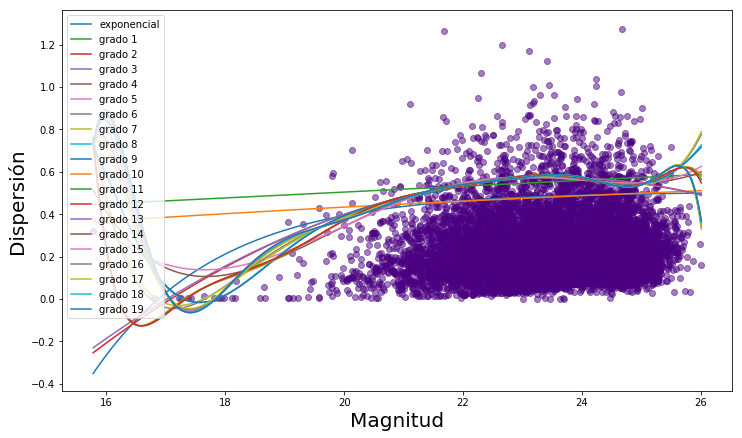
\includegraphics[scale = 0.6]{fits.png}
  \caption{Estrellas en el espacio de magnitud vs dispersión (usando cantidades robustas) junto a los modelos ya multiplicados por el threshold para buscar candidatos a estrellas variables }
  \label{figura}
\end{figure}

Tras elegir los mejores modelos, se decidió usar un polinomio de grado 13 para obtener la tendencia de los puntos y un threshold de 2.3. Se clasifica como candidatas a estrellas variables las estrellas por encima de la curva vista en la figura \ref{figura2}.

Se guarda el ID de las estrellas candidatas en un archivo \emph{candidatas.txt}. Debido al threshold utilizado y al modelo elegido, se encontró 3967 estrellas candidatas a estrellas variables. Casi el 40\% de las estrellas son candidatas a estrellas variables.

Todas las gráficas se hicieron en Python usando las librerías Matplotlib y Numpy.

\begin{figure}[ht!]
  \centering
   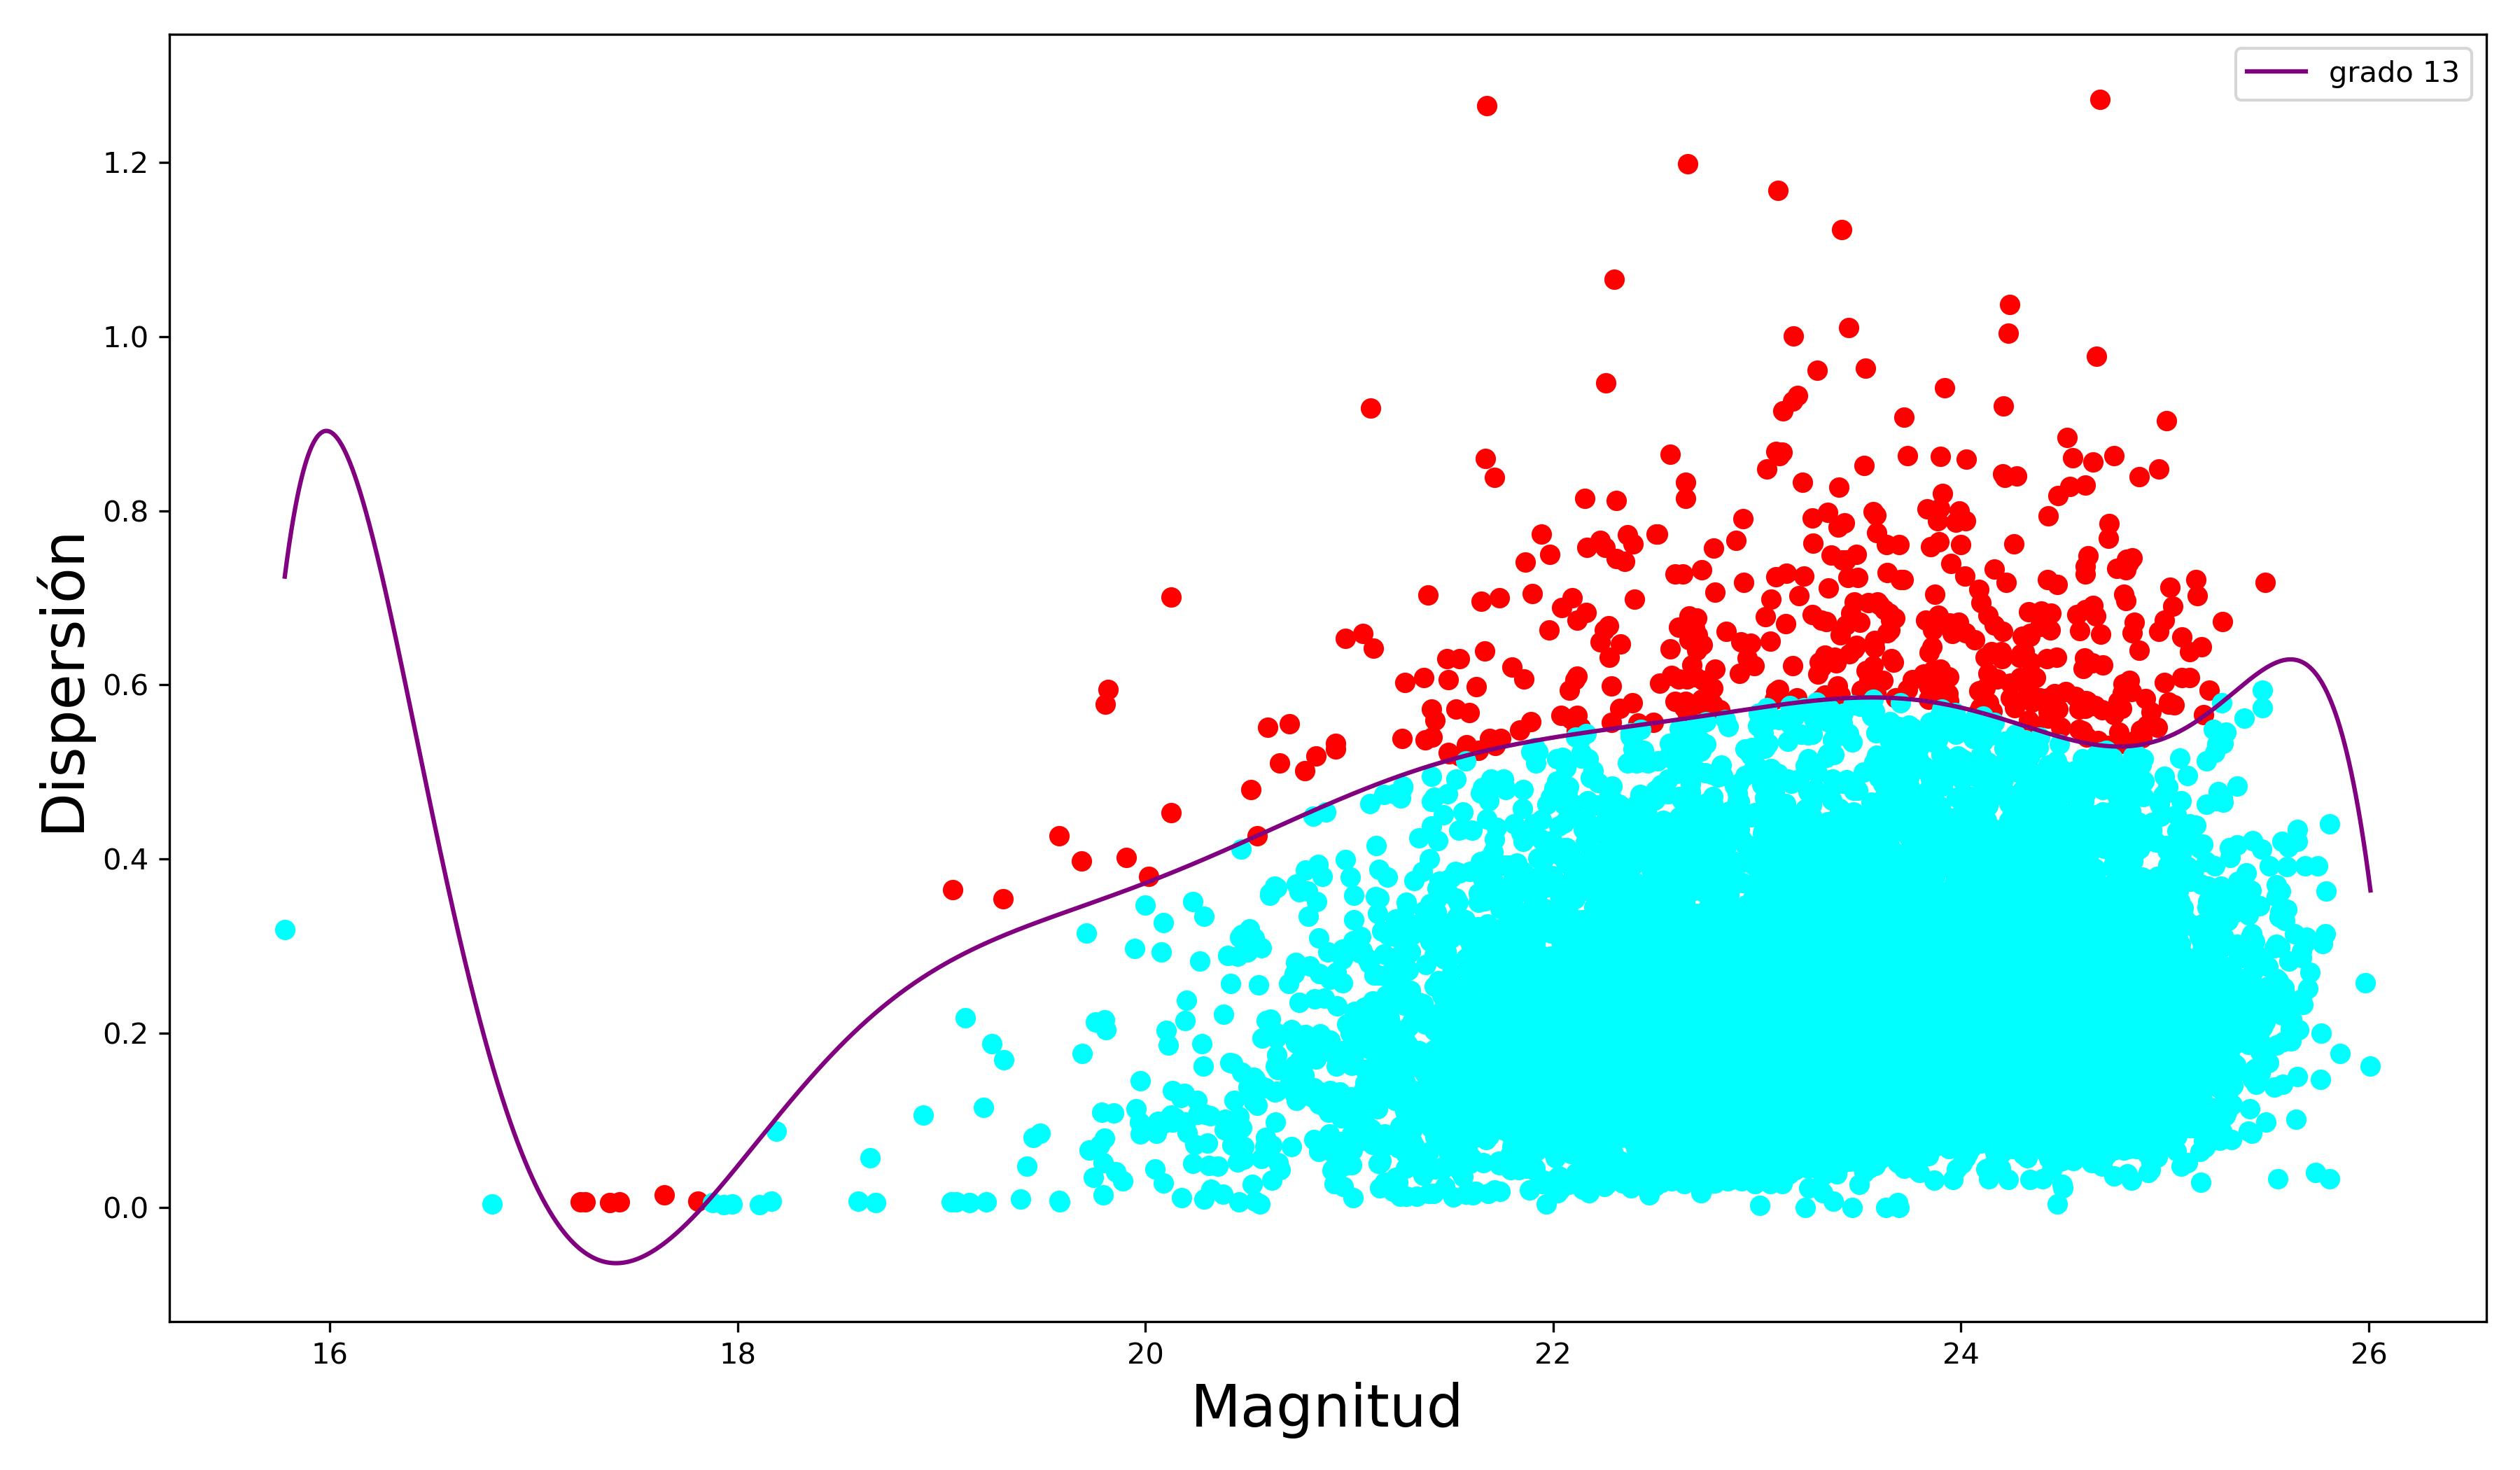
\includegraphics[scale = 0.6]{fits2.png}
  \caption{Estrellas en el espacio de magnitud vs dispersión (usando cantidades robustas) junto a los modelos ya multiplicados por el threshold para buscar candidatos a estrellas variables }
  \label{figura2}
\end{figure}


%\bibliography{bibte}
\bibliographystyle{plain}


\end{document}




\begin{figure}[H]
  \centering
   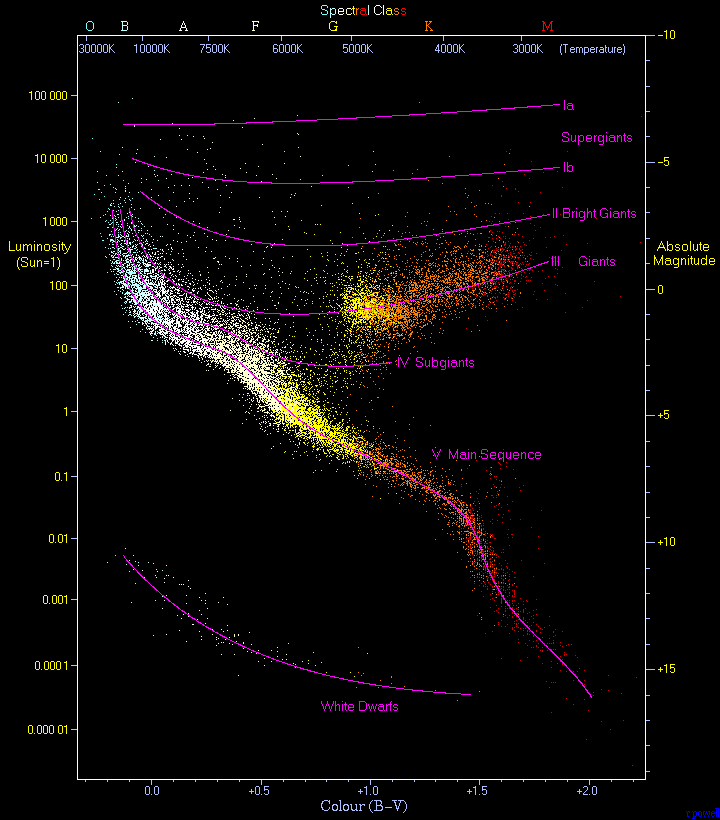
\includegraphics[width= 3.60in]{HRdiag.png}
  %\caption{Diagrama HR de 22000 estrellas del catálogo HIPPARCOS.\cite{hrdiag}  }
  \label{diag}
\end{figure}



\begin{table}[htb]
    \centering
    \label{tabla}
	\begin{tabular}{|c|c|c|c|c| }
	\hline
	Cúmulo & $E(B-V)$ & $m-M$ & Distancia [$pcs$] & Edad del cúmulo [millones de años]  \\ \hline
	NCG 752 & -0.03 & 8.02 & 401.79 & 1259  \\ \hline
	Mel 20 & +0.09 & 6.35 & 186.2 & 63  \\ \hline
	M45 & +0.04 & 5.50 & 125.89 & 126  \\ \hline
	Hyades & 0.00 & 2.84 & 36.98 & 891  \\ \hline
	M44 & +0.04 & 6.21 & 174.58 & 794  \\ \hline
	M67 & -0.03 & 9.32 & 731.14 & 5623  \\ \hline
	IC 4665 & 0.18 & 7.86 & 373.25 & 224  \\ \hline
	M39 & +0.01 & 6.87 & 238.78 & 447  \\ \hline
	\end{tabular}
\end{table}

\begin{table}[htb]
	\begin{tabular}{|c|cccccccccccccccc| }
	\hline
	Tareas $\backslash$ Semanas & 1 & 2 & 3 & 4 & 5 & 6 & 7 & 8 & 9 & 10 & 11 & 12 & 13 & 14 & 15 & 16  \\
	\hline
	1 & X & X & X  &   &   &   &   &  &  &   &   &   &   &   &   &   \\
	2 &   &  & X & X & X &  &  &   &   &  &  &  &   &  &  &   \\
	3 &   &   &   &  & X  & X  & X  & X &   &   &   &  &   &   &  &   \\
	4 &  &  &  &  &  &  &  & X & X & X & X &   &   &   &   &   \\
    5 &  &  &  &  &  &  & X & X &  &  &  &   &   &   &   &   \\
	6 &   &   &   &   &  &   &  X & X  &  &   &  X & X &  X & X  & X &   \\
	\hline
	\end{tabular}
\end{table}
\vspace{1mm}
%CCDRED se encarga de la corrección en sí, sus parámetros son: el tipo de dato de los pixeles (real, short, etc), el nombre del backup (en caso de querer un backup), el archivo de traducción del instrumento (que para una CCD estandar ya viene incluido en IRAF